\documentclass[../main.tex]{subfiles}
\graphicspath{{img/}}
\begin{document}
Da sempre l'uomo ha intuito che la materia, in tutta la sua varietà di forme, colori e consistenze, è il risultato della combinazione di pochi elementi fondamentali. Nel IV secolo a.C., Platone affermava che tutti i corpi sono solidi geometrici, definiti da superfici che è possibile ricoprire utilizzando soltanto triangoli isosceli e scaleni. Quindi questi triangoli sarebbero i costituenti fondamentali dei corpi, come le lettere dell'alfabeto sono i costituenti fondamentali delle sillabe e delle parole. Altri due filosofi dell'antica Grecia, Democrito e Leucippo, hanno introdotto il concetto di atomo come costituente fondamentale e indivisibile della materia. Specie diverse di atomi per forma geometrica e grandezza, conferiscono diverse proprietà alla materia.

Solo all'inizio del secolo scorso, grazie agli esperimenti di Dalton riguardo alle reazioni chimiche e alle teorie di Einstein sul moto Browniano, sono emerse le prime evidenze sull'esistenza degli atomi. La scoperta dell'elettrone da parte di Thomson nel 1897, dimostra l'esistenza di particelle più piccole dell'atomo, inaugurando la fisica nucleare.

\section{Esperimenti di diffusione}

\begin{figure}[tb]
    \centering
    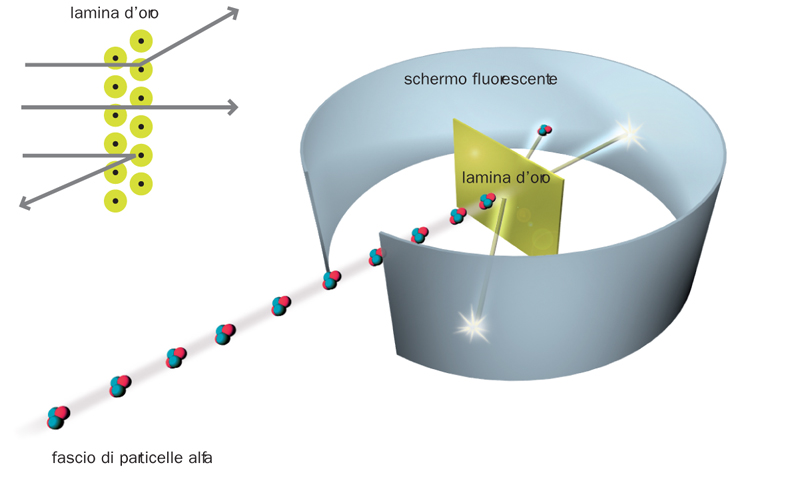
\includegraphics[width=\textwidth]{rutherford.jpg}
    \caption{L'esperimento ideato da Rutherford prevede un bersaglio d'oro di appena \SI{8.6e-6}{\cm} di spessore, irradiato da un flusso di particelle $\alpha$ generate dal decadimento di una lastra di radon. Il bersaglio è circondato da vetro dipinto con solfuro di zinco (ZnS), che scintilla al contatto con particelle cariche. Le particelle $\alpha$, cariche positivamente, in alcuni casi proseguono indisturbate e in altri vengono deviate a grandi angoli, fino anche ad essere respinte. Ciò dimostra l'inesattezza del modello atomico di Thomson, in cui la carica positiva dell'atomo ne riempie tutto il volume. Invece deve esistere all'interno dell'atomo una concentrazione di carica positiva abbastanza alta da poter deviare le pesanti particelle $\alpha$. \cite{as9_acdm}}
    \label{fig:rutherford}
\end{figure}

I primi esperimenti che hanno indagato la struttura interna dell'atomo sono quelli svolti da Rutherford, Geiger e Marsden tra il 1908 e il 1913, spinti nella loro ricerca dalle criticità del modello atomico sviluppato qualche anno prima da Thomson. Essi hanno utilizzato un flusso di particelle $\alpha$, i.e. nuclei di elio, di energia \SI{5.6}{\MeV} generate dal decadimento del radon, per bersagliare una foglia d'oro di spessore di appena \SI{8.6e-6}{\cm} (\autoref{fig:rutherford}). Intorno al bersaglio uno scintillatore composto da vetro dipinto con solfuro di zinco (ZnS) rendeva evidenti le particelle cariche prodotte dalla collisione. Come risultato, una certa percentuale di particelle $\alpha$ veniva deviata ad angoli molto maggiori di \SI{90}{°} o addirittura respinta, negando definitivamente il modello atomico di Thomson, che prevede un atomo mediamente neutro anche al proprio interno. Infatti, solo una grande concentrazione di carica poteva generare un campo elettrico capace di respingere le pesanti particelle $\alpha$. Si ipotizza quindi la presenza di un volume all'interno dell'atomo di dimensione molto minore dell'atomo stesso, in cui è concentrata tutta la carica di quest'ultimo: il nucleo. \mbox{Nasce così il modello atomico} planetario di Rutherford e le seguenti implicazioni che contribuirono all'origine della fisica quantistica.

Questo tipo di esperimento viene detto oggi \say{a target fisso}, per distinguerlo dai \emph{collisori} in cui due fasci di particelle diretti in direzioni opposte vengono fatti scontrare uno contro l'altro, e viene realizzato ancora nello stesso modo ideato da Rutherford: un fascio di particelle di opportuna energia viene scagliato contro un bersaglio a riposo nel sistema di riferimento dell'osservatore, e i prodotti della collisione sono rivelati con opportuna strumentazione.

L'invenzione e lo sviluppo degli acceleratori ha reso possibile selezionare e aumentare l'energia dei fasci e ridurne la dispersione energetica, parametri fondamentali per la buona riuscita degli esperimenti.
Infatti, da essa dipendono il potere risolutivo del fascio e la massa disponibile per la creazione di particelle.
A ciascuna particella di quantità di moto $p$ e energia $E$ è associata una lunghezza d'onda $\lambda = h / p $ dove $h$ è la costante di Planck, per il dualismo onda-particella, e una massa relativistica $m = E / c^2$ dove $c$ è la velocità della luce nel vuoto, per la relatività ristretta. 
Pensando l'onda-particella come una \say{nube} di probabilità, la lunghezza d'onda ne rappresenta le dimensioni. Quindi, il volume di questa \say{nube} può essere ristretto aumentando l'energia della particella. Maggiore l'energia, minore la lunghezza d'onda associata e minori le dimensioni degli oggetti con cui la particella può interagire. Inoltre, durante la collisione, l'energia delle particelle proiettile si deposita sul bersaglio e può eccitarne i nuclei. Questi, legati internamente dalla forza forte, dissipano l'energia producendo nuovi adroni. Maggiore l'energia, maggiore la massa disponibile.
Queste nuove particelle possono differire da quelle iniziali sia per natura, sia proprietà cinematiche. Inoltre, studiando le distribuzioni di questi stati finali, si possono ottenere informazioni sulla natura delle interazioni che sono intervenute nella collisione.

\section{Sezione d'urto}
Una delle grandezze fisiche che è possibile misurare in un esperimento di fascio di particelle a target fisso è il numero di particelle prodotte dall'interazione fascio-bersaglio nell'unità di tempo. Per esempio, nell'esperimento ideato da Rutherford, si tratta di contare le particelle $\alpha$ deflesse nell'unità di tempo, $\frac{\dd N_{def}}{\dd t}$. 
Questa frequenza è proporzionale al numero di particelle del fascio che arrivano sul bersaglio nell'unità di tempo, $\frac{\dd N_f}{\dd t}$, allo spessore $\Delta$x del bersaglio e alla densità di volume del bersaglio $n_b$
\begin{equation} \label{eq:def_ratio}
    \frac{\dd N_{def}}{\dd t} = \sigma_r \cdot \frac{\dd N_f}{\dd t} \cdot n_b \cdot \Delta \mathrm{x}
\end{equation}
Il fattore di proporzionalità $\sigma_r$ viene chiamato \emph{sezione d'urto} della reazione e ha le dimensioni di una superficie. Essa dipende dalla natura e dalle proprietà delle particelle che costituiscono fascio e bersaglio, oltre che dalla intensità della loro interazione. Di fatto, la sezione d'urto misura la probabilità che una certa interazione abbia luogo. Infatti, integrando la precedente equazione nel tempo, si ottiene 
\begin{equation}
    \sigma_r = \frac{N_{def}}{N_f} \frac{1}{n_b \cdot \Delta x}
\end{equation}
da cui è possibile determinare il valore della sezione d'urto della reazione. Si vede come la sezione d'urto sia proporzionale alla probabilità $\frac{N_{def}}{N_f}$.

La sezione d'urto è comunemente espressa in \emph{barn}, definito come
\begin{equation}
    1\ \mathrm{barn} = \SI{e-28}{\m ^2}
\end{equation}

Assumiamo ora un fascio con particelle distribuite in modo uniforme su una superficie $\Sigma$. L'equazione \ref{eq:def_ratio} può essere riscritta come 
\begin{equation}
    \frac{\dd N_{def}}{\dd t} = \sigma_r \cdot \phi \cdot N_b
\end{equation}
dove $\phi = \frac{\dd N_f}{\dd t \cdot \Sigma}$ è il flusso di particelle del fascio per unità di tempo e unità di superficie, e $N_b = n_b \cdot \Sigma \cdot \Delta \mathrm{x}$ è il numero di particelle del bersaglio illuminate dal fascio. 

Il flusso $\phi$ può essere espresso attraverso la densità e la velocità dei proiettili. Infatti, il numero di proiettili può essere scritto come $\dd N_f = n_f \Sigma \cdot v \dd t$ dove $v$ è la velocità del fascio. Quindi 
\begin{equation}
    \phi = \frac{n_f \Sigma \cdot v \dd t}{\dd t \cdot \Sigma} = n_f \cdot v
\end{equation}

\section{Raggi cosmici}

\begin{figure}[!b]
    \centering
    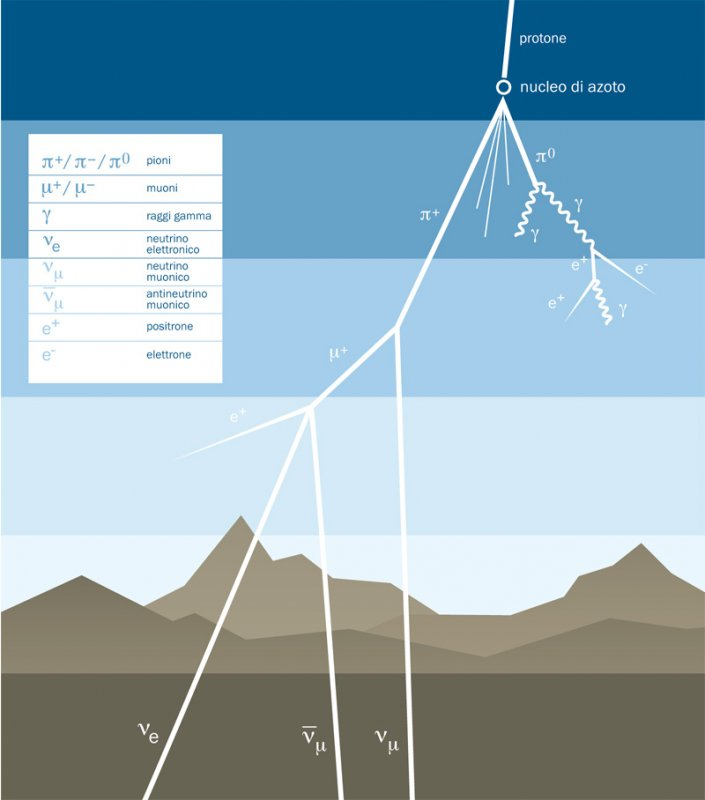
\includegraphics[width=0.7\textwidth]{cosmic.jpg}
    \caption{Rappresentazione pittorica delle reazioni generate dall'ingresso di un protone cosmico nell'atmosfera. I pioni carichi, prodotti dalla collisione tra protoni e nuclei atomici nell'atmosfera terrestre, decadono in neutrini e muoni e quest'ultimi in ulteriori neutrini e elettroni, realizzando così una \emph{cascata adronica}. I pioni neutri, invece, decadono in una coppia di fotoni, ciascuno dei quali può decadere in una coppia elettrone-positrone. A loro volta elettroni e positroni possono produrre fotoni come radiazione di frenamento, innescando così reazioni a catena dette \emph{cascata elettromagnetica}.
    \cite{as10_vdu}}
    \label{fig:cosmic}
\end{figure}

Prima dell'invenzione degli acceleratori, avvenuta nel secondo Novecento, la fisica delle particelle aveva come unico ambito lo studio delle radiazioni ionizzanti prodotte da fenomeni naturali.
Nel 1912, Hess mostra la presenza di una radiazione di origine extraterrestre, i raggi cosmici, rilevando come l'intensità di radiazione ionizzante cresce all'aumentare dell'altitudine.

Di origine galattica e extragalattica (\emph{Active Galactic Nuclei}, \emph{Gamma Ray Bursts}), i raggi cosmici (\autoref{fig:cosmic}) sono composti principalmente da protoni ($85\%$), nuclei di elio ($12\%$), nuclei pesanti ($1\%$) e elettroni ($2\%$). Interagendo coi nuclei dell'atmosfera terrestre in collisioni ad alta energia ($1 -$\SI{e10}{\GeV}), essi generano una radiazione secondaria costituita da pioni, mesoni-K e altri adroni più pesanti. Questi a loro volta, se hanno abbastanza energia, possono produrre altri adroni nell'interazione coi nuclei atomici nell'atmosfera terreste, realizzando quella che viene definita una \emph{cascata adronica}. 
Inizialmente il numero di particelle prodotte nella cascata aumenta fino ad arrestarsi quando l'energia delle particelle si riduce al di sotto della soglia energetica per la formazione di nuove particelle ($E_{th} = m_{0}c^2$).
\mbox{Infatti gli adroni prodotti sono instabili.} I pioni carichi decadono con vita media di appena \SI{26}{\ns} (a riposo) in muoni, a loro volta instabili con vita media (a riposo) di \SI{2}{\micro\s}. I pioni neutri invece, decadono tramite interazione elettromagnetica in una coppia di fotoni, i quali, interagendo coi nuclei dell'atmosfera, generano elettroni e positroni. Questi emettono a loro volta fotoni come radiazione di frenamento, realizzando così una \emph{cascata elettromagnetica}.


In conclusione, a Terra riceviamo principalmente due componenti della radiazione cosmica: una \emph{soft}, composta dalla cascata elettromagnetica, la quale viene assorbita da materiali come il piombo, e una \emph{hard}, composta principalmente da muoni, la quale è in grado di penetrare anche strati spessi di materia. 
Una terza componente, estremamente difficile da rivelare, è costituita dai neutrini prodotti dal decadimento degli adroni e dei muoni cosmici in elettroni.

\section{Scintillatori}
Una delle tecniche più usate per rivelare il passaggio di particelle cariche è sfruttare la ionizzazione del mezzo che attraversano. In particolare, esistono materiali chiamati \say{scintillatori} che presentano caratteristiche ideali. 
Si possono distinguere due categorie di materiali scintillatori.
\emph{Organici}, ovvero composti aromatici come il benzene, caratterizzati da un tempo di risposta di pochi nanosecondi. Possono essere in forma di cristallo (come l'\emph{anthracene}), liquida o plastica. \emph{Inorganici}, ovvero cristalli alcalini come lo ioduro di sodio. Questo tipo di scintillatore ha grande efficienza luminosa, i.e. produce molti fotoni per quantità di radiazione ionizzante, ma ha tempi di risposta più lenti degli scintillatori di tipo organico.

I rivelatori a scintillazione (\autoref{fig:pmt}) raccolgono i fotoni emessi dallo scintillatore e li incanalano in un fotomoltiplicatore, il quale produce elettroni per effetto fotoelettrico e li converte in segnale elettrico. Il tutto è protetto da un materiale che scherma da campi magnetici esterni, come quello terrestre.

\begin{figure}[!b]
    \centering
    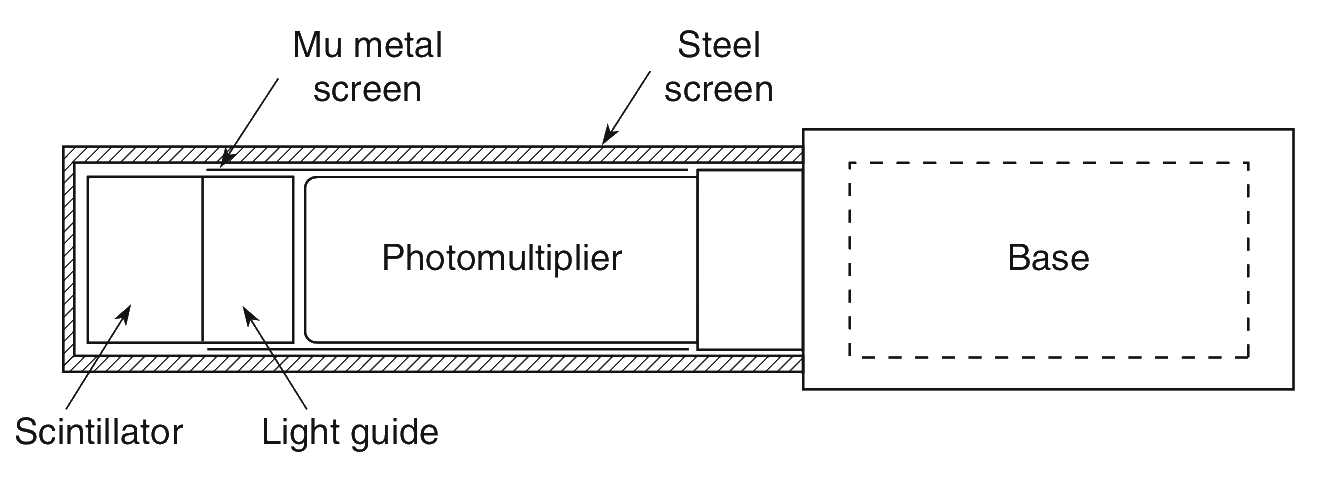
\includegraphics[width=\textwidth]{pmt_trasp.png}
    \caption{Lo schema di un rivelatore a scintillazione. Quando una radiazione ionizzante entra nello scintillatore, ne eccita gli atomi i quali, diseccitandosi, emettono fotoni. Questi entrano nel fotomoltiplicatore dove vengono convertiti in segnale elettrico tramite effetto fotoelettrico. Uno strato di materiale ferromagnetico (\emph{mu-metal}: \SI{80}{\%} nickel, \SI{20}{\%} ferro) scherma da campi magnetici come quello terrestre.
    \cite{spurio}}
    \label{fig:pmt}
\end{figure}


Tipicamente si usano tubi fotomoltiplicatori costituiti da una serie di dinodi, ciascuno con potenziale maggiore del precedente. All'ingresso del fotomoltiplicatore, un catodo viene colpito dai fotoni prodotti dallo scintillatore ed emette elettroni per effetto fotoelettrico, i quali vengono attratti dal primo dinodo della serie a causa della differenza di potenziale. Da qui, un maggior numero di elettroni vengono attirati verso il dinodo successivo per \emph{emissione secondaria}. Quindi, un anodo raccoglie gli elettroni al termine della serie di dinodi, per un fattore totale di moltiplicazione di \SI{e5}{} $-$ \SI{e7}{}.

\end{document}
